\section*{Supplemental Materials}
\subsection*{Sampled Nearby Mutational Landscape}\label{ss:sampled_nearby}
As noted in equation \ref{eq:phenotypic_diffusion_rate}, the mutants in the nearby mutational landscape include those that have more than one mutation. However, for completeness, we performed an exhaustive landscaping of the single-step mutational landscape, which, by definition, only includes mutants with a single mutation (see Figure \ref{fig:CCE_single_step}). In order to verify that our results are indeed representative of the expected genomic and phenotypic diffusion rates, we sampled the mutants in the nearby mutational landscape using all naturally occurring mutations, including multiple mutations in a single mutant.

%=[FIGURE - Frac 1-step vs Frac Sampled]
	\begin{figure}[!h] %% FIGURE 6
	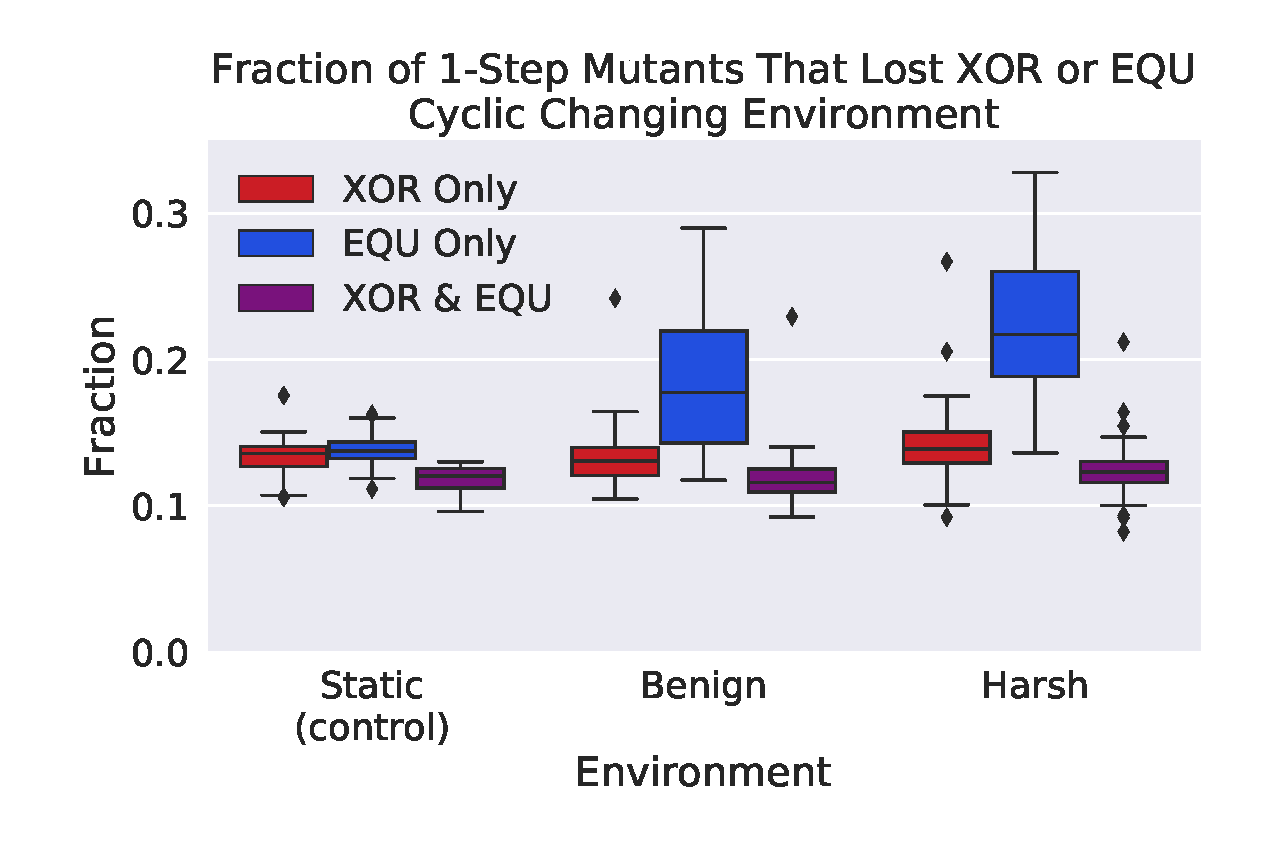
\includegraphics[width=0.95\columnwidth]{figures/CE/fig10.eps}
    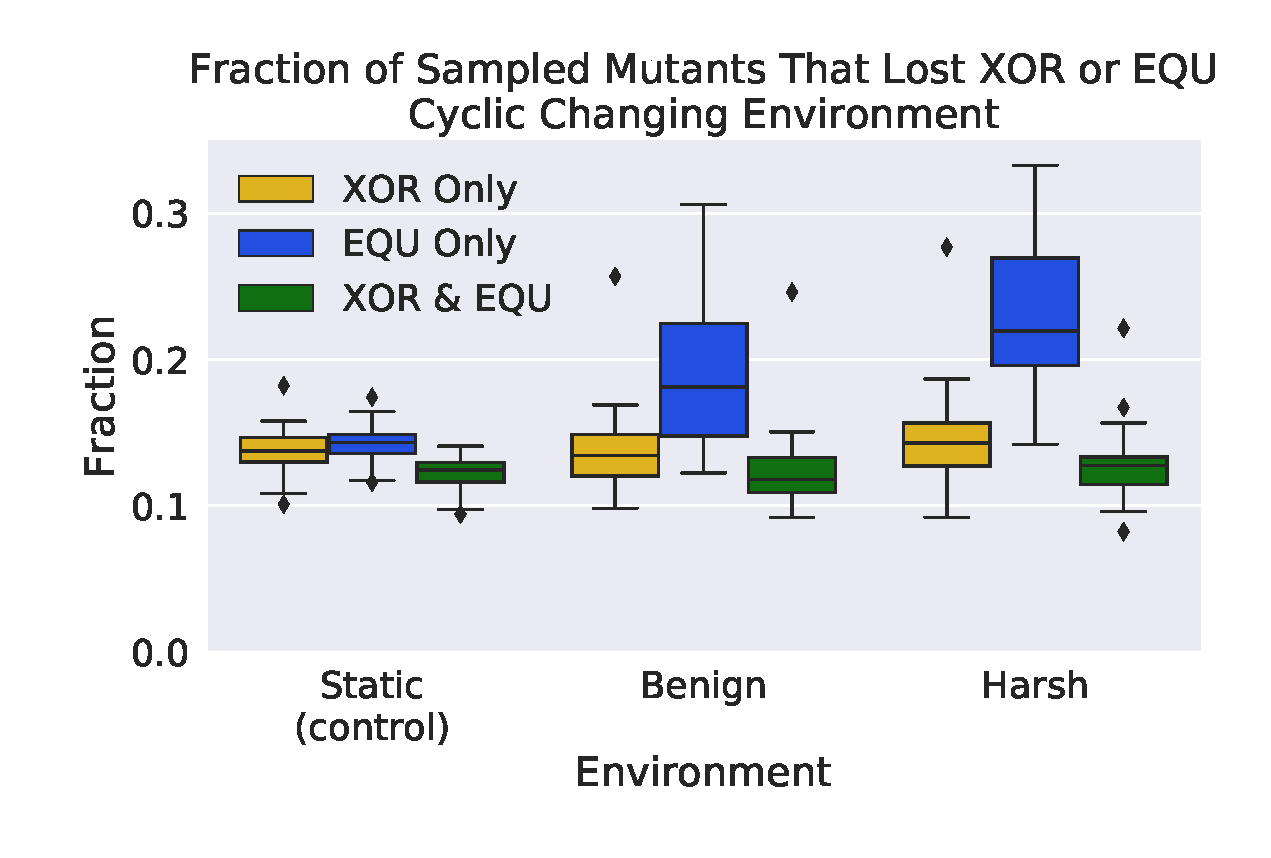
\includegraphics[width=0.95\columnwidth]{figures/CE/figA.eps}
	\caption{\textbf{A survey of the single-step and sampled mutational neighborhoods} around organisms that performed the fluctuating task. The results are qualitatively identical to each other.   
	}\label{fig:CCE_sample_step}
	\end{figure}

Our results (see figure \ref{fig:CCE_sample_step})  were virtually identical, showing that the sampling approach and the exhaustive landscaping produce qualitatively indistinguishable results.